\chapter{Results And Analysis} \label{c:tc2} 
This chapter presents the experimental results across all configurations and models.

\section{Single-Device Performance Baseline (RQ1)}
This section compares single-device inference performance between llama.cpp (C1) and Distributed Llama (C2) across tier A and B models on a single Raspberry Pi 5 (16 GB).

\subsection{Tier A Models: Small Models on a Single Device}
Table 4.1 and 4.2 present the performance for the tier A models.
\begin{table}[H]
    \centering
    \begin{tabular}{|>{\raggedright\arraybackslash}p{1.5cm}|>{\raggedright\arraybackslash}p{2cm}|>{\raggedright\arraybackslash}p{1.5cm}|>{\raggedright\arraybackslash}p{1.5cm}|>{\raggedright\arraybackslash}p{1.5cm}|>{\raggedright\arraybackslash}p{1.5cm}|>{\raggedright\arraybackslash}p{1.5cm}|>{\raggedright\arraybackslash}p{1.5cm}|}\hline
         Prompt&  Config&  Gen Rate (tok/s)&  PP Rate tok/s&  TTFT (ms)&  E2E Latency (ms)&  CPU (\%)& Mem (MB)\\\hline
         P01&  llama.cpp&  14.72&  90.60&  200.4&  3,482&  59.5& 5,620\\\hline
         P02&  llama.cpp&  13.88&  139.24&  366.5&  36,533&  92.0& 5,624\\\hline
         P03&  llama.cpp&  13.61&  138.81&  2,033.3&  5,579&  70.2& 5,653\\\hline
         P04&  llama.cpp&  13.25&  140.78&  2,298.9&  36,305&  91.3& 5,659\\\hline
 \textbf{AVG}& \textbf{llama.cpp}& \textbf{13.87}& \textbf{127.36}& \textbf{1,224.8}& \textbf{20,475}& \textbf{78.3}&\textbf{5,639}\\\hline
         P01&  dllama&  15.71&  16.75&  754.5&  9,461&  49.6& 3,104\\\hline
         P02&  dllama&  14.27&  16.92&  1,999.5&  42,873&  88.3& 3,164\\\hline
         P03&  dllama&  13.89&  16.44&  2,000.5&  31,126&  83.4& 3,054\\\hline 
 P04& dllama& 13.38& 16.15& 2,010.0& 36,113& 85.5&3,113\\ \hline
 \textbf{AVG}& \textbf{dllama}& \textbf{14.31}& \textbf{16.56}& \textbf{1,691.1}& \textbf{29,893}& \textbf{76.7}&\textbf{3,109}\\\hline
    \end{tabular}
    \caption{Llama 3.2 1B Instruct Q4\_0 - Single Device Performance}
    \label{tab:placeholder}
\end{table}

\begin{table}[H]
    \centering
    \begin{tabular}{|>{\raggedright\arraybackslash}p{1.5cm}|>{\raggedright\arraybackslash}p{2cm}|>{\raggedright\arraybackslash}p{1.5cm}|>{\raggedright\arraybackslash}p{1.5cm}|>{\raggedright\arraybackslash}p{1.5cm}|>{\raggedright\arraybackslash}p{1.5cm}|>{\raggedright\arraybackslash}p{1.5cm}|>{\raggedright\arraybackslash}p{1.5cm}|}\hline
         Prompt&  Config&  Gen Rate (tok/s)&  PP Rate tok/s&  TTFT (ms)&  CPU (\%)& Mem (MB)\\\hline
         P01&  llama.cpp&  11.07&  54.92&  290.8&    65.6& 6,458\\\hline
         P02&  llama.cpp&  9.97&  95.66&  518.6&    94.2& 6,461\\\hline
         P03&  llama.cpp&  9.79&  92.10&  3,044.7&    75.8& 6,487\\\hline
         P04&  llama.cpp&  9.11&  92.98&  3,465.4&    93.7& 6,491\\\hline
         \textbf{AVG}&  \textbf{llama.cpp}&  \textbf{9.98}&  \textbf{83.92}&  \textbf{1,829.9}&  \textbf{82.3}& \textbf{6,474}\\\hline
         P01&  dllama&  11.67&  12.38&  928.0&    81.1& 2,297\\\hline
         P02&  dllama&  9.97&  12.41&  2,695.5&    98.1& 2,325\\\hline 
         P03& dllama& 9.79& 11.86& 2,732.5&  97.2&2,294\\ \hline
         P04& dllama& 9.14& 11.52& 2,731.5& 98.1&2,308\\\hline
         \textbf{AVG}& \textbf{dllama}& \textbf{10.14}& \textbf{12.04}& \textbf{2,271.9}&  \textbf{93.6}&\textbf{2,306}\\\hline
    \end{tabular}
    \caption{Qwen3 1.7B Q4\_0 - Single Device Performance}
    \label{tab:placeholder}
\end{table}
Token generation rates were similar between the two frameworks. For Llama 3.2 1B, llama.cpp achieved 13.87 tok/s and Distributed Llama achieved 14.31 tok/s. For Qwen3 1.7B, the rates were also similar at 9.98 tok/s versus 10.14 tok/s. These results fall within the 5-15 tok/s range that Nguyen \cite{RN3} reported for the models in the 1B-1.5B parameter range.

Despite these comparable generation speeds, Distributed Llama reported a much lower prompt processing rate than llama.cpp (around 16 tok/s versus 127-141 tok/s). The reason lies in their implementations. Even though both frameworks split the prompt into chunks and run the model once per chunk, they use different chunk sizes. The llama.cpp processes the prompt in chunks of 512 tokens while Distributed Llama uses chunks of only 32 tokens. For a 350 token prompt, llama.cpp requires a single pass, whereas Distributed Llama requires eleven passes. Chunk size matters because of how matrix multiplication performs on a CPU. A larger chunk means a larger matrix multiplication per forward pass, resulting at a better rate. The difference of 16x smaller explains the gap in prompt processing rate. Another difference is in how Distributed count time, it only counts time spent inside the model excluding the scheduling overhead between chunk, while llama.cpp includes everything. Thus, the two numbers are not comparable. Since both measure the TTFT in the similar way, it is the reliable metric for comparing the two framework performance.

Distributed Llama used noticeably less memory than llama.cpp, around 3.1GB vs 5.6GB for Llama 3.2 1B, and 2.3 GB vs 6.5 GB for Qwen 3 1.7B. This was surprising because Distributed Llama pins its weights in RAM with \verb|mlock()| while llama.cpp lets the operating system page weights in and out as needed. Thus, Distributed Llama should use more memory, not less than llama.cpp. This behavior is due to when a context is created, llama.cpp immediately reserves the full key-value cache at the maximum configured context length and pre-allocates worst-case compute buffers at the context initialization to cover the maximum intermediate activation that any operation in its compute graph might produce. Both stay resident for the entire session. Specifically, Qwen3 1.7B is only about 2.2 GB on disk, but llama.cpp's memory reached 6.5 GB, the extra memory 4.2 GB was mostly from these pre-allocated buffers. On the other hand, Distributed Llama takes a different approach, in which it declares a fixed set of small activation buffers for its batch size of 32, not worse case, and share across all layers. For Qwen3 model, these buffers only cost tens of megabytes, whereas llama.cpp's buffer is several gigabytes. 

CPU utilization showed an interesting pattern. For short output prompts, CPU utilization was moderate, while for long output prompts, it approached saturation at 92-98 \%. This shows that the CPU is not continuously saturated during the prompt processing phase instead it reaches full utilization during the autoregressive generation phase, which is consistent with Berglund \cite{RN12} findings.


\subsection{Tier B Models: Medium Models Under Memory Pressure}
\begin{table}[H]
    \centering
    \begin{tabular}{|>{\raggedright\arraybackslash}p{1.5cm}|>{\raggedright\arraybackslash}p{2cm}|>{\raggedright\arraybackslash}p{1.5cm}|>{\raggedright\arraybackslash}p{1.5cm}|>{\raggedright\arraybackslash}p{1.5cm}|>{\raggedright\arraybackslash}p{1.5cm}|>{\raggedright\arraybackslash}p{1.5cm}|>{\raggedright\arraybackslash}p{1.5cm}|}\hline
         Prompt&  Config&  Gen Rate (tok/s)&  PP Rate tok/s&  TTFT (ms)&  CPU (\%)& Mem (MB)\\\hline
         P01&  llama.cpp&  -&  -&  -&  -&  OOM\\\hline
         P02&  llama.cpp&  -&  -&  -&  -&  OOM\\\hline
         P03&  llama.cpp&  -&  -&  -&  -&  OOM\\\hline
         P04&  llama.cpp&  -&  -&  -&  -&  OOM\\\hline
         P01&  dllama& 2.50& 2.60&  4,638.0&  54.8& 13,878\\\hline
         P02&  dllama& 2.20& 2.65&  3,449.5&  93.7& 13,901\\\hline 
         P03&  dllama& 2.10& 2.41&  7,015.0& 93.7& 13,739\\\hline 
         P04&  dllama& 2.00& 2.39&  131,161.7& 93.2& 13,619\\\hline
         \textbf{AVG}& \textbf{dllama}& \textbf{2.20}& \textbf{2.51}& \textbf{36,566.0}& \textbf{83.8}&  \textbf{13,784}\\\hline
    \end{tabular}
    \caption{Llama 3.1 8B Instruct Q4\_0 - Single Device Performance}
    \label{tab:placeholder}
\end{table}
\begin{table}[H]
    \centering
    \begin{tabular}{|>{\raggedright\arraybackslash}p{1.5cm}|>{\raggedright\arraybackslash}p{2cm}|>{\raggedright\arraybackslash}p{1.5cm}|>{\raggedright\arraybackslash}p{1.5cm}|>{\raggedright\arraybackslash}p{1.5cm}|>{\raggedright\arraybackslash}p{1.5cm}|>{\raggedright\arraybackslash}p{1.5cm}|>{\raggedright\arraybackslash}p{1.5cm}|}\hline
         Prompt&  Config&  Gen Rate (tok/s)&  PP Rate tok/s&  TTFT (ms)&  CPU (\%)& Mem (MB)\\\hline
         P01&  llama.cpp&  2.71&  8.29&  1,698.1&  81.9& 14,072\\\hline
         P02&  llama.cpp&  2.57&  20.34& 2,355.5&  97.2& 14,077\\\hline
         P03&  llama.cpp&  2.56&  19.97& 13,961.3& 87.2& 14,129\\\hline
         P04&  llama.cpp&  2.46&  21.04& 15,234.8& 96.8& 14,137\\\hline
         \textbf{AVG}& \textbf{llama.cpp}& \textbf{2.57}& \textbf{17.41}& \textbf{8,312.4}& \textbf{90.8}&  \textbf{14,104}\\\hline
         P01&  dllama& 2.34& 2.66& 4,204.5& 81.6& 12,735\\\hline
         P02&  dllama& 2.13& 2.51& 3,291.5& 98.7& 12,791\\\hline 
         P03&  dllama& 2.03& 2.33& 6,723.5& 97.9& 12,049\\\hline 
         P04&  dllama& 1.99& 2.31& 135,257.0& 98.6& 11,880\\\hline
         \textbf{AVG}& \textbf{dllama}& \textbf{2.12}& \textbf{2.45}& \textbf{37,369.1}& \textbf{94.2}&  \textbf{12,364}\\\hline
    \end{tabular}
    \caption{Qwen3 8B Q4\_0 - Single Device Performance}
    \label{tab:placeholder}
\end{table}

It was interesting to see that the Llama 3.1 8B went out of memory (OOM) when running under llama.cpp while running successfully under Distributed Llama. This OOM failure is due to the differences in model formats and memory management between frameworks that is discussed in the tier A analysis. This OOM behavior challenges the assumption in the existing literature \cite{RN12, RN3} that model file size alone determines single-device feasibility.

On the other hand, the Qwen3 8B model worked well under two frameworks. The performance also followed tier A pattern but with lower throughput. Given that llama.cpp achieved 2.57 tok/s versus Distributed Llama's 2.12 tok/s, both fall within the 1-3 tok/s range that Berglund \cite{RN12} reported. The prompt processing gap persisted at tier B. Specifically, llama.cpp processed prompt at 17.41 tok/s compared to Distributed Llama's 2.45 tok/s. This gap was even worse for large model since the absolute values are already low. 

Regarding the memory usage, llama.cpp used about 16 GB while Distributed Llama used 12 GB, which were within the memory limit of the Raspberry Pi 5. Also, for generation-heavy prompts, both frameworks reached 90\% CPU utilization.

\subsection{Summary}
The single-device evaluation revealed three key findings for RQ1.

First, token generation rates were nearly identical between the two frameworks across all tested models. Tier A models achieved approximately 10-14 tok/s, within Nguyen's \cite{RN3} reported range, while Tier B models dropped to 2-3 tok/s, consistent with Berglund's \cite{RN12} findings. Neither framework had an advantage in the autoregressive generation phase.

Second, Distributed Llama consistently used less resident memory than llama.cpp due to llama.cpp's pre-allocation of the full KV cache and worst-case compute buffers at context initialization. This difference was critical in practice where Llama 3.1 8B crashed with out-of-memory errors under llama.cpp but ran successfully under Distributed Llama on the same hardware. This challenges the assumption in existing literature \cite{RN12, RN3} that model file size alone determines single-device feasibility.

Third, CPU utilization reached 92-98\% during token generation but remained moderate during prompt processing, confirming that the generation phase is compute-bound while the pre-fill phase is memory-bandwidth-bound.

In practical terms, Distributed Llama's lower memory footprint makes it the only viable option for running 8B-class models on the 16 GB Raspberry Pi 5, while llama.cpp offers more efficient prompt processing for models that fit comfortably within memory.

\section{Distributed Inference Viability and Overhead (RQ2)}
\begin{table}[H]
 \centering
    \begin{tabular}{|>{\raggedright\arraybackslash}p{1.5cm}|>{\raggedright\arraybackslash}p{2cm}|>{\raggedright\arraybackslash}p{1.5cm}|>{\raggedright\arraybackslash}p{1.5cm}|>{\raggedright\arraybackslash}p{1.5cm}|>{\raggedright\arraybackslash}p{1.5cm}|>{\raggedright\arraybackslash}p{1.5cm}|>{\raggedright\arraybackslash}p{1.5cm}|}\hline
Prompt & Config& Eval tok/s & Prompt tok/s & TTFT (ms) & CPU (\%) & Mem (MB) \\ \hline
P01 & llama.cpp&12.36 & 26.58 & 532.4 & 19.8 & 818 \\ \hline
P02 & llama.cpp&10.91 & 27.97 & 1,557.6 & 26.1 & 818 \\ \hline
P03 & llama.cpp&10.92 & 27.77 & 9,960.6 & 20.3 & 818 \\ \hline
P04 & llama.cpp&10.08 & 27.81 & 11,351.5 & 24.6 & 818 \\ \hline
\textbf{AVG} & \textbf{llama.cpp}& \textbf{11.07} & \textbf{27.53} & \textbf{5,850.5} & \textbf{22.7} & \textbf{818} \\ \hline
P01 & dllama&24.45 & 27.84 & 378.0 & 28.5 & 3,625 \\ \hline
P02 & dllama&23.16 & 28.87 & 987.5 & 75.5 & 3,625 \\ \hline
P03 & dllama&22.69 & 28.78 & 1,011.0 & 71.1 & 3,625 \\ \hline
P04 & dllama&22.65 & 28.76 & 988.0 & 70.5 & 3,625 \\ \hline
\textbf{AVG} & \textbf{dllama}&\textbf{23.24} & \textbf{28.56} & \textbf{841.1} & \textbf{61.4} & \textbf{3,625} \\ \hline
\end{tabular}
\caption{Llama 3.2 1B Instruct Q4\_0 (Tier A)}
\end{table}

\begin{table}[H]
 \centering
    \begin{tabular}{|>{\raggedright\arraybackslash}p{1.5cm}|>{\raggedright\arraybackslash}p{2cm}|>{\raggedright\arraybackslash}p{1.5cm}|>{\raggedright\arraybackslash}p{1.5cm}|>{\raggedright\arraybackslash}p{1.5cm}|>{\raggedright\arraybackslash}p{1.5cm}|>{\raggedright\arraybackslash}p{1.5cm}|>{\raggedright\arraybackslash}p{1.5cm}|}\hline
Prompt & Config& Eval tok/s & Prompt tok/s & TTFT (ms) & CPU (\%) & Mem (MB) \\ \hline
P01 & llama.cpp&8.91 & 17.29 & 748.6 & 20.3 & 1,240 \\ \hline
P02 & llama.cpp&8.25 & 18.71 & 2,258.9 & 27.3 & 1,240 \\ \hline
P03 & llama.cpp&8.01 & 18.82 & 14,629.4 & 21.7 & 1,240 \\ \hline
P04 & llama.cpp&7.62 & 18.72 & 16,797.5 & 25.9 & 1,240 \\ \hline
\textbf{AVG} & \textbf{llama.cpp}&\textbf{8.20} & \textbf{18.38} & \textbf{8,608.6} & \textbf{23.8} & \textbf{1,240} \\ \hline
P01 & dllama&18.79 & 19.41 & 485.0 & 38.9 & 3,915 \\ \hline
P02 & dllama&17.16 & 20.94 & 1,333.0 & 86.7 & 3,915 \\ \hline
P03 & dllama&16.55 & 20.51 & 1,330.0 & 82.9 & 3,915 \\ \hline
P04 & dllama&16.53 & 20.50 & 1,331.5 & 82.7 & 3,915 \\ \hline
\textbf{AVG} & \textbf{dllama}& \textbf{17.26} & \textbf{20.34} & \textbf{1,119.9} & \textbf{72.8} & \textbf{3,915} \\ \hline
\end{tabular}
\caption{Qwen3 1.7B Q4\_0 (Tier A)}
\end{table}

\begin{table}[H]
 \centering
    \begin{tabular}{|>{\raggedright\arraybackslash}p{1.5cm}|>{\raggedright\arraybackslash}p{2cm}|>{\raggedright\arraybackslash}p{1.5cm}|>{\raggedright\arraybackslash}p{1.5cm}|>{\raggedright\arraybackslash}p{1.5cm}|>{\raggedright\arraybackslash}p{1.5cm}|>{\raggedright\arraybackslash}p{1.5cm}|>{\raggedright\arraybackslash}p{1.5cm}|}\hline
Prompt & Config& Eval tok/s & Prompt tok/s & TTFT (ms) & CPU (\%) & Mem (MB) \\ \hline
P01 & llama.cpp& 2.08 & 3.79 & 3,650.3 & 13.6 & 6,833 \\ \hline
P02 & llama.cpp& 2.00 & 3.94 & 10,915.9 & 24.3 & 6,833 \\ \hline
P03 & llama.cpp& 1.99 & 3.91 & 70,510.1 & 18.7 & 6,833 \\ \hline
P04 & llama.cpp& 1.93 & 3.92 & 80,299.4 & 23.6 & 6,833 \\ \hline
\textbf{AVG} & \textbf{llama.cpp}& \textbf{2.00} & \textbf{3.89} & \textbf{41,343.9} & \textbf{20.0} & \textbf{6,833} \\ \hline
P01 & dllama&4.53 & 4.91 & 2,357.5 & 34.6 & 11,264 \\ \hline
P02 & dllama&4.26 & 4.83 & 6,508.5 & 82.8 & 11,264 \\ \hline
P03 & dllama&4.04 & 4.56 & 6,545.0 & 80.3 & 11,264 \\ \hline
P04 & dllama&4.00 & 4.52 & 6,497.0 & 80.3 & 11,264 \\ \hline
\textbf{AVG} & \textbf{dllama}& \textbf{4.21} & \textbf{4.70} & \textbf{5,477.0} & \textbf{69.5} & \textbf{11,264} \\ \hline
\end{tabular}
\caption{Llama 3.1 8B Instruct Q4\_0 (Tier B)}
\end{table}

\begin{table}[H]
 \centering
    \begin{tabular}{|>{\raggedright\arraybackslash}p{1.5cm}|>{\raggedright\arraybackslash}p{2cm}|>{\raggedright\arraybackslash}p{1.5cm}|>{\raggedright\arraybackslash}p{1.5cm}|>{\raggedright\arraybackslash}p{1.5cm}|>{\raggedright\arraybackslash}p{1.5cm}|>{\raggedright\arraybackslash}p{1.5cm}|>{\raggedright\arraybackslash}p{1.5cm}|}\hline
Prompt & Config& Eval tok/s & Prompt tok/s & TTFT (ms) & CPU (\%) & Mem (MB) \\ \hline
P01 & llama.cpp&2.22 & 3.63 & 3,476.3 & 19.2 & 5,101 \\ \hline
P02 & llama.cpp&2.11 & 3.90 & 10,727.9 & 24.9 & 5,101 \\ \hline
P03 & llama.cpp&2.08 & 3.93 & 69,964.6 & 21.2 & 4,930 \\ \hline
P04 & llama.cpp&2.02 & 3.94 & 79,794.3 & 24.3 & 5,101 \\ \hline
\textbf{AVG} & \textbf{llama.cpp}&\textbf{2.11} & \textbf{3.85} & \textbf{40,990.8} & \textbf{22.4} & \textbf{5,058} \\ \hline
P01 & dllama& 4.71 & 5.01 & 2,040.0 & 39.1 & 11,084 \\ \hline
P02 & dllama& 4.16 & 5.11 & 6,072.5 & 87.1 & 11,084 \\ \hline
P03 & dllama& 3.97 & 4.59 & 6,169.0 & 85.0 & 11,084 \\ \hline
P04 & dllama& 3.93 & 4.52 & 6,201.0 & 84.9 & 11,084 \\ \hline
\textbf{AVG} & \textbf{dllama}& \textbf{4.19} & \textbf{4.81} & \textbf{5,120.6} & \textbf{74.0} & \textbf{11,084} \\ \hline
\end{tabular}
\caption{Qwen3 8B Q4\_0 (Tier B)}
\end{table}
\subsection{Generation Rate}

\begin{figure}[htbp]
  \centering
  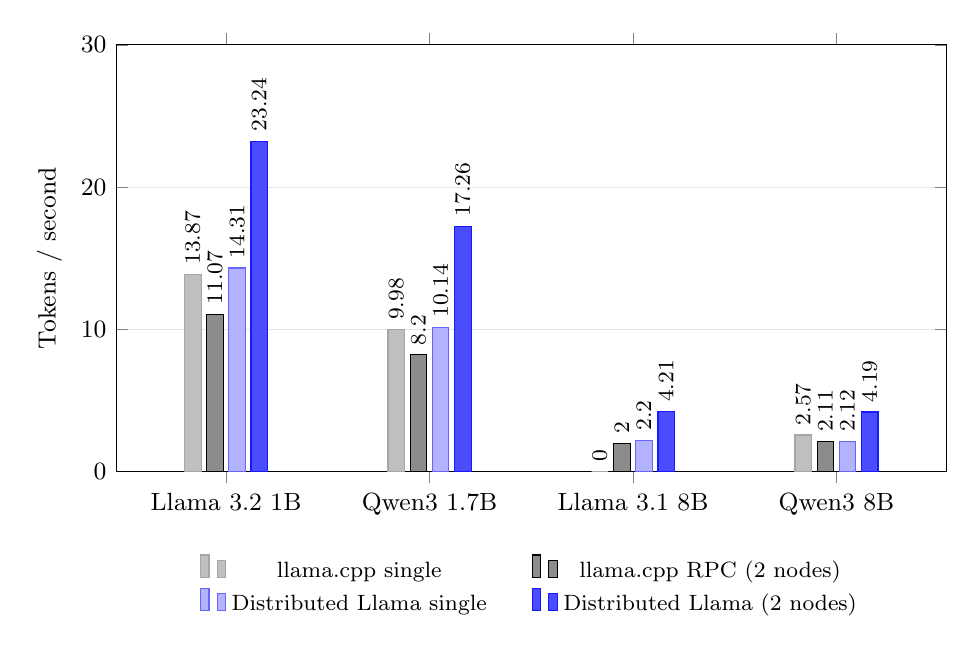
\begin{tikzpicture}
    \begin{axis}[
        ybar,
        bar width=6pt,
        width=\linewidth,
        height=7cm,
        enlarge x limits=0.18,
        ymin=0, ymax=30,
        ylabel={Tokens / second},
        symbolic x coords={Llama 3.2 1B, Qwen3 1.7B, Llama 3.1 8B, Qwen3 8B},
        xtick=data,
        xticklabel style={font=\small},
        yticklabel style={font=\small},
        ylabel style={font=\small},
        nodes near coords,
        every node near coord/.append style={
            font=\footnotesize, 
            rotate=90, 
            anchor=west,
            /pgf/number format/fixed,
            /pgf/number format/precision=2
        },
        legend style={
          at={(0.5,-0.18)}, anchor=north,
          legend columns=2, font=\footnotesize, draw=none,
          /tikz/every even column/.append style={column sep=0.5cm},
        },
        ymajorgrids, major grid style={gray!20},
    ]
      \addplot[fill=gray!50, draw=gray!70] coordinates {
        (Llama 3.2 1B,13.87) (Qwen3 1.7B,9.98) (Llama 3.1 8B,0) (Qwen3 8B,2.57)};
      \addplot[fill=gray!90, draw=black] coordinates {
        (Llama 3.2 1B,11.07) (Qwen3 1.7B,8.20) (Llama 3.1 8B,2.00) (Qwen3 8B,2.11)};
      \addplot[fill=blue!30, draw=blue!60] coordinates {
        (Llama 3.2 1B,14.31) (Qwen3 1.7B,10.14) (Llama 3.1 8B,2.20) (Qwen3 8B,2.12)};
      \addplot[fill=blue!70, draw=blue!90] coordinates {
        (Llama 3.2 1B,23.24) (Qwen3 1.7B,17.26) (Llama 3.1 8B,4.21) (Qwen3 8B,4.19)};
      \legend{llama.cpp single, llama.cpp RPC (2 nodes), Distributed Llama single, Distributed Llama (2 nodes)}
    \end{axis}
  \end{tikzpicture}
  \caption{Token generation rate across configurations. Llama 3.1~8B under llama.cpp single-device is omitted (OOM). Distributed Llama on 2 nodes nearly doubles throughput on the 8B-class models, while llama.cpp RPC pays an 18--20\% pipeline-bubble penalty.}
  \label{fig:rq2-genrate}
\end{figure}

The two frameworks behaved differently when moving from single node to two nodes. For llama.cpp RPC, the results showed a reduction in token generation rate. Specifically, Llama 3.2 1B dropped from 13.87 tok/s on a single device to 11.07 tok/s across two nodes, approximately 20\%. Qwen3 1.7B and Qwen 38B showed the same pattern. Yet, this is expected from pipeline parallelism on a \textbf{single request} workloads. Since each layer group depends on the activations produced by the preceding group, only one node at any given time works while the other waits. The network hop between stages also adds overhead. The pipeline bubble mentioned in Section 2.5.2 is therefore not a theoretical concern, but a real problem.

Distributed Llama, on the other hand, showed a better trend. Specifically, Llama 3.2 1B accelerated from 14.31 tok/s to 23.24 tok/s, approximately 64\%. Qwen3 1.7B, Qwen 3 8B and Llama 3.1 8B also showed the same pattern. Fro the 8B-class models, two nodes delivered almost exactly the doubling that tensor parallelism predicts in theory. This indicates that the communication cost per layer is small enough compared to the per-layer compute on Raspberry Pi 5.
\subsection{Time to First Token}

\begin{figure}[htbp]
  \centering
  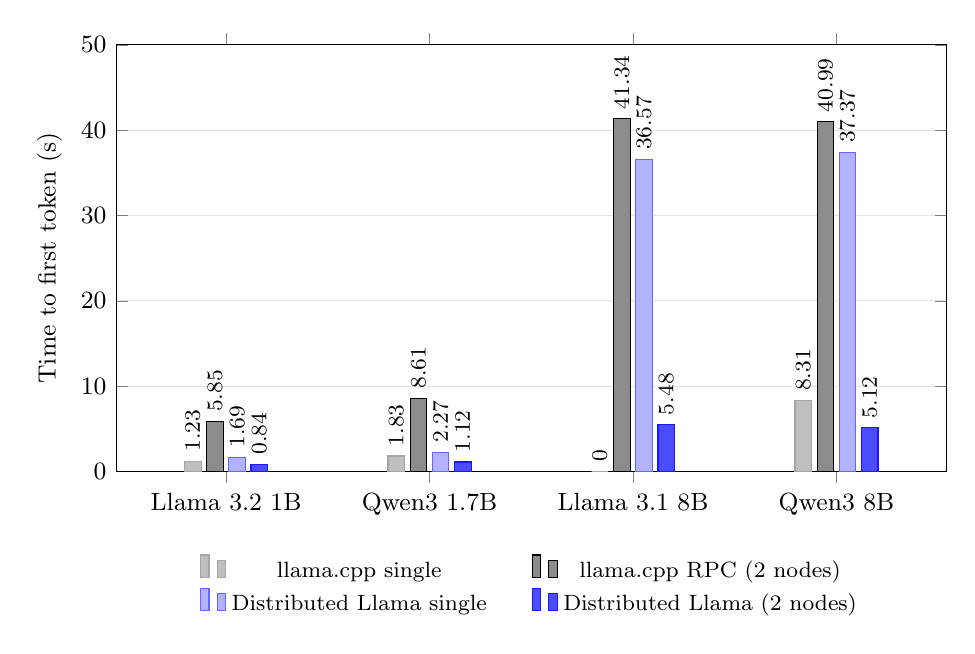
\begin{tikzpicture}
     \begin{axis}[
        ybar,
        bar width=6pt,
        width=\linewidth,
        height=7cm,
        enlarge x limits=0.18,
        ymin=0, ymax=50,
        ylabel={Time to first token (s)},
        symbolic x coords={Llama 3.2 1B, Qwen3 1.7B, Llama 3.1 8B, Qwen3 8B},
        xtick=data,
        xticklabel style={font=\small},
        yticklabel style={font=\small},
        ylabel style={font=\small},
        nodes near coords,
        every node near coord/.append style={
            font=\footnotesize, 
            rotate=90, 
            anchor=west,
            /pgf/number format/fixed,
            /pgf/number format/precision=2
        },
        legend style={
          at={(0.5,-0.18)}, anchor=north,
          legend columns=2, font=\footnotesize, draw=none,
          /tikz/every even column/.append style={column sep=0.5cm},
        },
        ymajorgrids, major grid style={gray!20},
    ]
      \addplot[fill=gray!50, draw=gray!70] coordinates {
        (Llama 3.2 1B,1.225) (Qwen3 1.7B,1.830) (Llama 3.1 8B,0) (Qwen3 8B,8.312)};
      \addplot[fill=gray!90, draw=black] coordinates {
        (Llama 3.2 1B,5.851) (Qwen3 1.7B,8.609) (Llama 3.1 8B,41.344) (Qwen3 8B,40.991)};
      \addplot[fill=blue!30, draw=blue!60] coordinates {
        (Llama 3.2 1B,1.691) (Qwen3 1.7B,2.272) (Llama 3.1 8B,36.566) (Qwen3 8B,37.369)};
      \addplot[fill=blue!70, draw=blue!90] coordinates {
        (Llama 3.2 1B,0.841) (Qwen3 1.7B,1.120) (Llama 3.1 8B,5.477) (Qwen3 8B,5.121)};
      \legend{llama.cpp single, llama.cpp RPC (2 nodes), Distributed Llama single, Distributed Llama (2 nodes)}
    \end{axis}
  \end{tikzpicture}
  \caption{Average time to first token.}
  \label{fig:rq2-ttft}
\end{figure}

The TTFT results reinforced this difference. For llama.cpp RPC, the average TTFT roughly quadrupled to quintupled when moving to two nodes. Pipeline parallelism does not improve the performance for a single request workload in any way. The prompt still flows through the layer sequentially with extra latency due to network hop. In contrast, Distributed Llama reduced TTFT substantially across all models. This is because tensor parallelism splits the matrix multiplications used in prompt processing across both nodes in the same way it splits the generation step, so the pre-fill phase benefits from parallel compute as well.

\subsection{Per-Node Memory}

\begin{figure}[htbp]
  \centering
  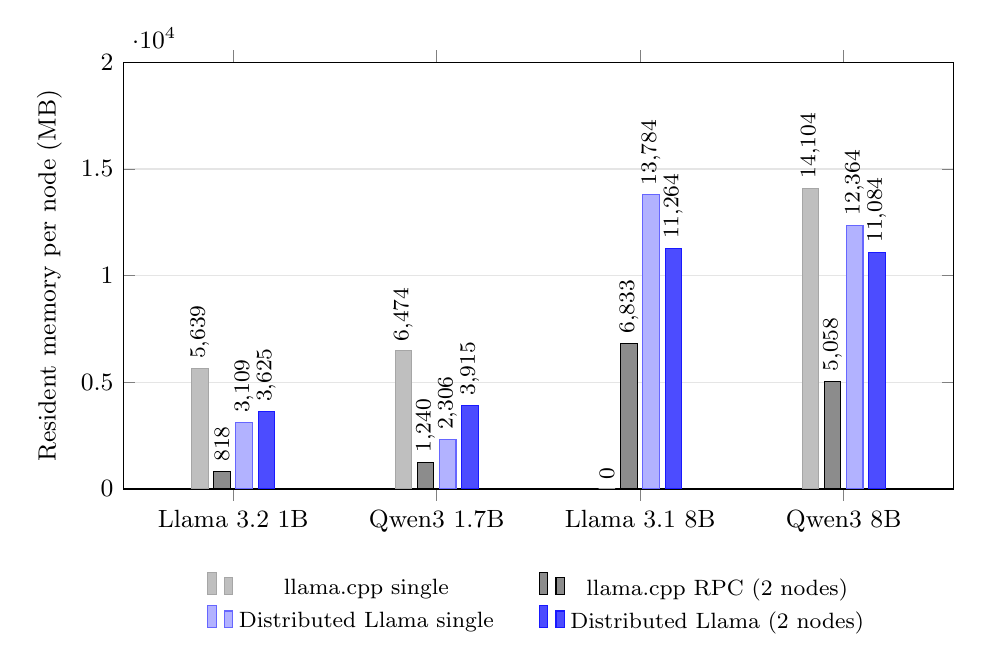
\begin{tikzpicture}
    \begin{axis}[
        ybar,
        bar width=6pt,
        width=\linewidth,
        height=7cm,
        enlarge x limits=0.18,
        ymin=0, ymax=20000,
        ylabel={Resident memory per node (MB)},
        symbolic x coords={Llama 3.2 1B, Qwen3 1.7B, Llama 3.1 8B, Qwen3 8B},
        xtick=data,
        xticklabel style={font=\small},
        yticklabel style={font=\small},
        ylabel style={font=\small},
        nodes near coords,
        every node near coord/.append style={
            font=\footnotesize, 
            rotate=90, 
            anchor=west,
            /pgf/number format/fixed,
            /pgf/number format/precision=2
        },
        legend style={
          at={(0.5,-0.18)}, anchor=north,
          legend columns=2, font=\footnotesize, draw=none,
          /tikz/every even column/.append style={column sep=0.5cm},
        },
        ymajorgrids, major grid style={gray!20},
    ]
      \addplot[fill=gray!50, draw=gray!70] coordinates {
        (Llama 3.2 1B,5639) (Qwen3 1.7B,6474) (Llama 3.1 8B,0) (Qwen3 8B,14104)};
      \addplot[fill=gray!90, draw=black] coordinates {
        (Llama 3.2 1B,818) (Qwen3 1.7B,1240) (Llama 3.1 8B,6833) (Qwen3 8B,5058)};
      \addplot[fill=blue!30, draw=blue!60] coordinates {
        (Llama 3.2 1B,3109) (Qwen3 1.7B,2306) (Llama 3.1 8B,13784) (Qwen3 8B,12364)};
      \addplot[fill=blue!70, draw=blue!90] coordinates {
        (Llama 3.2 1B,3625) (Qwen3 1.7B,3915) (Llama 3.1 8B,11264) (Qwen3 8B,11084)};
      \legend{llama.cpp single, llama.cpp RPC (2 nodes), Distributed Llama single, Distributed Llama (2 nodes)}
    \end{axis}
  \end{tikzpicture}
  \caption{Resident memory per node}
  \label{fig:rq2-memory}
\end{figure}

In the single-device experiments, llama.cpp could not load Llama 3.1 8B because of its pre-allocated KV cache and worse-case compute buffers. The Qwen3 8B while working also consumed roughly 14GB of memory. Pooling memory across two nodes solved both cases. Both models ran successfully under both frameworks, with the memory consumed within the 16GB ceiling. Thus, pooling memory across two nodes validates the premise of the RQ2 which claims it helps run models that a single device cannot host.

\subsection{Cost of Distribution}
The overhead of distribution question posed in RQ2 had two different answers depending on which framework is used. For pipeline parallelism via llama.cpp RPC, the overhead was significant, an 18\%-20\% reduction in throughput and 4-5x increase in TTFT. For tensor parallelism via Distributed Llama, the distribution instead produced a 60-90\% speedup in throughput and reduction. As a result, the cost of distribution when using Distributed Llama was negative.

\subsection{Summary}
These findings answer the RQ2 directly. Firstly, distributed inference is possible on Raspberry Pi 5 hardware connected via Gigabit Ethernet. Both frameworks completed all Tier A and Tier B workloads including the 8B-class models that exceeded the single-device limits when using llama.cpp. Secondly, the cost of the distribution heavily depends on the parallelism strategy. Specifically, pipeline parallelism showed an extra latency on the single request case due to the I/O waiting, while the tensor parallelism delivered near-linear speedup since the per-layer compute latency dominates all the all-reduce communication cost. Finally, the experiment showed that using Raspberry Pi 5 cluster with Distributed Llama could improve the performance of 8B-class models from approximately 2 tok/s (nearly OOM on a single device) to 4 tok/s, comfortably fitting within the cluster's memory. This finding validates the premise of this thesis that distributed inference is a viable alternative to cloud offloading for IoT use cases with modest throughput.

\section{Framework Comparison (RQ3)}
\begin{table}[H]
 \centering
    \begin{tabular}{|>{\raggedright\arraybackslash}p{1.5cm}|>{\raggedright\arraybackslash}p{2cm}|>{\raggedright\arraybackslash}p{1.5cm}|>{\raggedright\arraybackslash}p{1.5cm}|>{\raggedright\arraybackslash}p{1.5cm}|>{\raggedright\arraybackslash}p{1.5cm}|>{\raggedright\arraybackslash}p{1.5cm}|>{\raggedright\arraybackslash}p{1.5cm}|}\hline
Prompt & Config & Eval tok/s & Prompt tok/s & TTFT (ms) & CPU (\%) & Mem (MB) \\ \hline
P01 & llama.cpp& 1.22 & 1.95 &  6461.1&   14.6&    8790 \\ \hline
P02 & llama.cpp& 1.17 & 2.08 &  20127.9&   23.8&   8790 \\ \hline
P03 & llama.cpp& 1.16 & 2.09 & 131475.0&  21.0&   8790 \\ \hline
P04 & llama.cpp& 1.13 & 2.09 & 149950.6&  23.8&   8790 \\ \hline
\textbf{AVG} & \textbf{llama.cpp}& \textbf{1.17} & \textbf{2.05} & \textbf{77003.65} & \textbf{20.8} & \textbf{8790} \\ \hline
P01 & dllama & 2.36 & 2.31 & 4,611.0 & 25.2 & 14,679 \\ \hline
P02 & dllama & 2.15 & 2.31 & 3,336.5 & 72.9 & 14,602 \\ \hline
P03 & dllama & 2.06 & 2.29 & 7,579.0 & 68.4 & 15,535 \\ \hline
P04 & dllama & 2.12 & 2.37 & 72,083.3 & 68.1 & 15,110 \\ \hline
\textbf{AVG} & \textbf{dllama}& \textbf{2.17} & \textbf{2.32} & \textbf{21,902.5} & \textbf{58.7} & \textbf{14,982} \\ \hline
\end{tabular}
\caption{Qwen3 14B Q4\_0 (Tier C)}
\end{table}

\subsection{Generation Rate}
\begin{figure}[htbp]
  \centering
  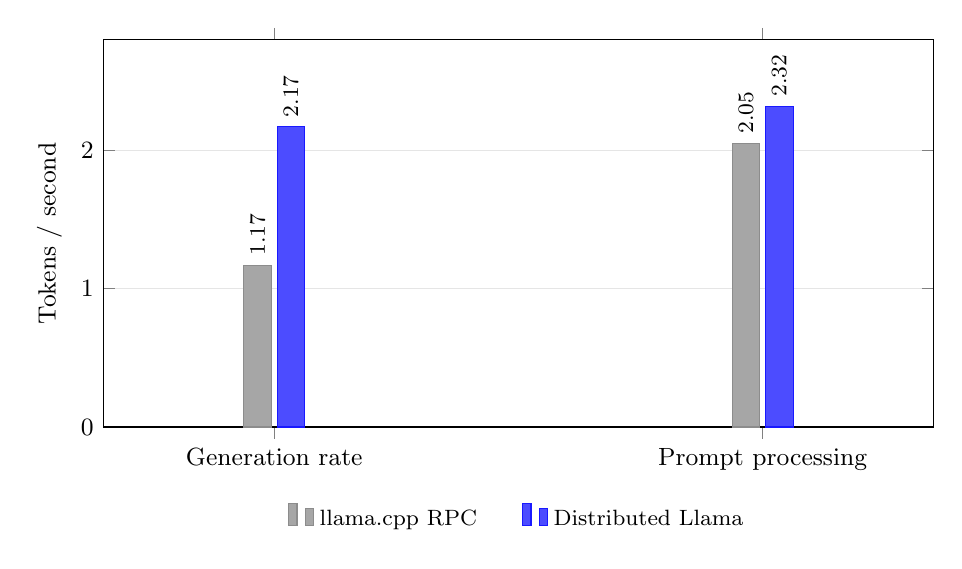
\begin{tikzpicture}
    \begin{axis}[
        ybar,
        bar width=10pt,
        width=\linewidth,
        height=6.5cm,
        enlarge x limits=0.35,
        ymin=0, ymax=2.8,
        ylabel={Tokens / second},
        symbolic x coords={Generation rate, Prompt processing},
        xtick=data,
        xticklabel style={font=\small},
        yticklabel style={font=\small},
        ylabel style={font=\small},
        nodes near coords,
        every node near coord/.append style={
            font=\footnotesize, 
            rotate=90, 
            anchor=west,
            /pgf/number format/fixed,
            /pgf/number format/precision=2
        },
        legend style={
          at={(0.5,-0.18)}, anchor=north,
          legend columns=2, font=\footnotesize, draw=none,
          /tikz/every even column/.append style={column sep=0.5cm},
        },
        ymajorgrids, major grid style={gray!20},
    ]
      \addplot[fill=gray!70, draw=gray!90] coordinates {
        (Generation rate,1.17) (Prompt processing,2.05)};
      \addplot[fill=blue!70, draw=blue!90] coordinates {
        (Generation rate,2.17) (Prompt processing,2.32)};
      \legend{llama.cpp RPC, Distributed Llama}
    \end{axis}
  \end{tikzpicture}
  \caption{Throughput comparison on Qwen3 14B Q4\_0.} 
  \label{fig:rq3-throughput}
\end{figure}

Distributed Llama had an average of 2.17 tok/s compared to llama.cpp RPC's 1.17 tok/s, which was an 85\% faster. This result extends the tier B findings that the compute dominates communication on Raspberry Pi 5 hardware. 

\subsection{Time to First Token}
TTFT followed the same pattern as generation rate. Specifically, Distributed Llama averaged 21.9 seconds compared to llama.cpp RPC's 77.0 seconds, a roughly 3.5x faster. For long prompts under llama.cpp RPC, P03 and P04, the time was too large, 131 and 149 seconds, and might not be acceptable for the IoT application defined in Section 1.2. On the other hand, Distributed Llama's 21.0 seconds on average was closer to usable, though the value 72 seconds on P04 showed that long input workloads remain inefficient at 14B regardless of framework.
\begin{figure}[H]
  \centering
  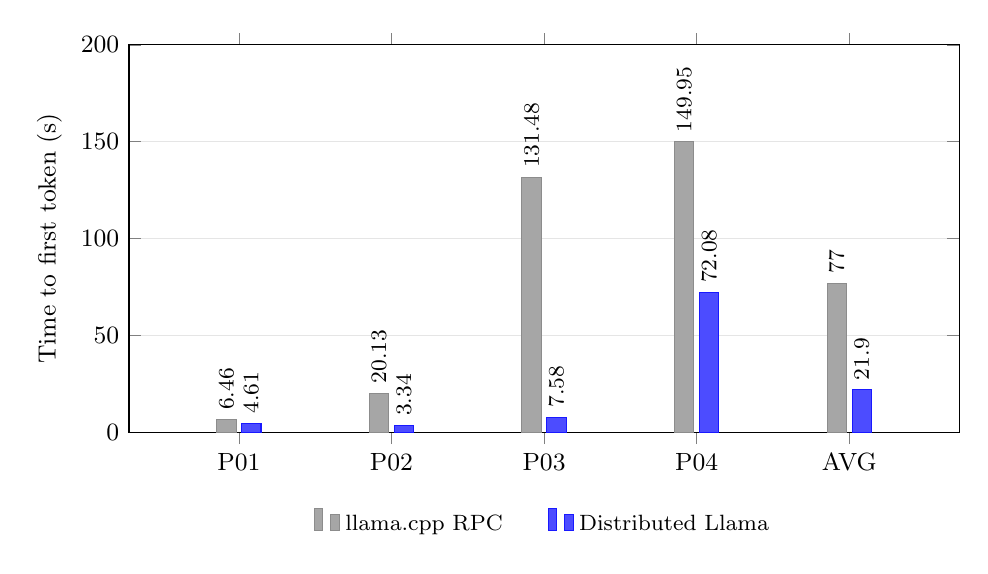
\begin{tikzpicture}
    \begin{axis}[
        ybar,
        bar width=7pt,
        width=\linewidth,
        height=6.5cm,
        enlarge x limits=0.18,
        ymin=0, ymax=200,
        ylabel={Time to first token (s)},
        symbolic x coords={P01, P02, P03, P04, AVG},
        xtick=data,
        % Keeping the data labels so the exact numbers are still easy to read
        nodes near coords,
        every node near coord/.append style={
            font=\footnotesize, 
            rotate=90, 
            anchor=west,
            /pgf/number format/fixed,
            /pgf/number format/precision=2
        },
        xticklabel style={font=\small},
        yticklabel style={font=\small},
        ylabel style={font=\small},
        legend style={
          at={(0.5,-0.18)}, anchor=north,
          legend columns=2, font=\footnotesize, draw=none,
          /tikz/every even column/.append style={column sep=0.5cm},
        },
        ymajorgrids, major grid style={gray!20},
    ]
      \addplot[fill=gray!70, draw=gray!90] coordinates {
        (P01,6.46) (P02,20.13) (P03,131.48) (P04,149.95) (AVG,77.00)};
      \addplot[fill=blue!70, draw=blue!90] coordinates {
        (P01,4.61) (P02,3.34) (P03,7.58) (P04,72.08) (AVG,21.90)};
      \legend{llama.cpp RPC, Distributed Llama}
    \end{axis}
  \end{tikzpicture}
  \caption{Time to first token per prompt on Qwen3 14B Q4\_0 (lower is better).}
  \label{fig:rq3-ttft}
\end{figure}


\subsection{CPU Utilization}
\begin{figure}[htbp]
  \centering
  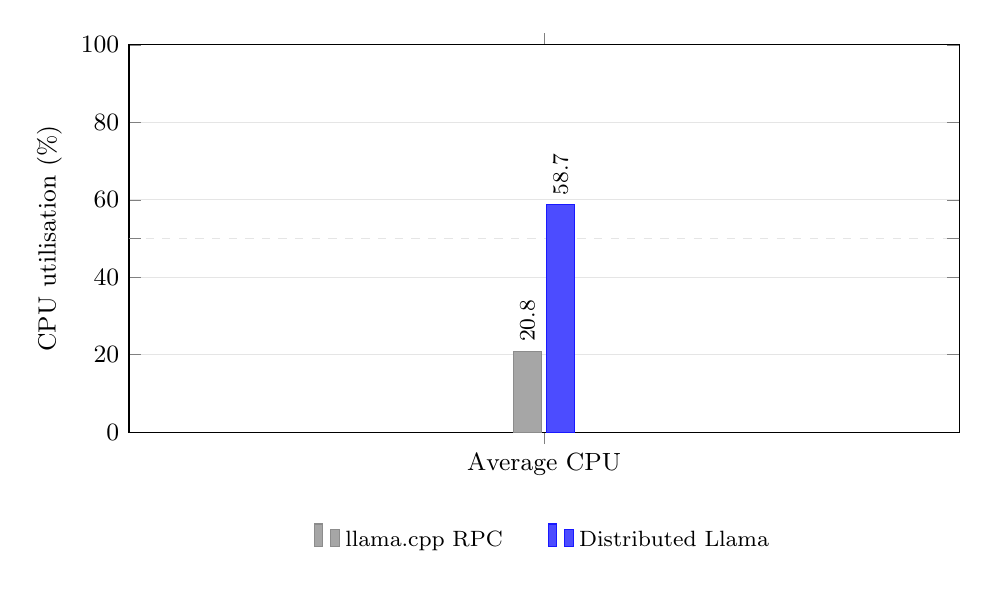
\begin{tikzpicture}
    \begin{axis}[
        ybar,
        bar width=10pt,
        width=\linewidth,
        height=6.5cm,
        enlarge x limits=0.5,
        ymin=0, ymax=100,
        ylabel={CPU utilisation (\%)},
        symbolic x coords={Average CPU},
        xtick=data,
        xticklabel style={font=\small},
        yticklabel style={font=\small},
        ylabel style={font=\small},
        nodes near coords,
        every node near coord/.append style={
            font=\footnotesize, 
            rotate=90, 
            anchor=west,
            /pgf/number format/fixed,
            /pgf/number format/precision=2
        },
        legend style={
          at={(0.5,-0.22)}, anchor=north,
          legend columns=2, font=\footnotesize, draw=none,
          /tikz/every even column/.append style={column sep=0.5cm},
        },
        ymajorgrids, major grid style={gray!20},
        extra y ticks={50},
        extra y tick style={grid=major, grid style={dashed, gray!40}, tick label style={font=\tiny, color=gray}},
        extra y tick labels={},
    ]
      \addplot[fill=gray!70, draw=gray!90] coordinates {(Average CPU,20.8)};
      \addplot[fill=blue!70, draw=blue!90] coordinates {(Average CPU,58.7)};
      \legend{llama.cpp RPC, Distributed Llama}
    \end{axis}
  \end{tikzpicture}
  \caption{Average CPU utilisation during inference on Qwen3 14B Q4\_0}
  \label{fig:rq3-cpu}
\end{figure}
The llama.cpp RPC averaged only 20.8\% CPU utilization during inference while Distributed Llama reached 58.7\%. In theory, on a 2-node cluster processing single request, each node should spend roughly half its time waiting for the other to finish computing. The result confirms this behavior. Neither framework was fully using the hardware, but Distributed Llama kept both nodes three times busier than llama.cpp RPC does.

\subsection{Prompt Processing Rate}
At tier A, llama.cpp performed much better than Distributed Llama, 127 tok/s compared to 16 tok/s. However, at tier C, the gap was gone. The reason is that the larger chunk size of llama.cpp only matters when matrix multiplication throughput is the bottleneck. At 14B, per-token compute is so heavy that the scheduling overhead becomes relatively small. This means the prompt processing advantage of llama.cpp on small models does not generalize to the larger models. 

\subsection{Per-Node Memory}
\begin{figure}[htbp]
  \centering
  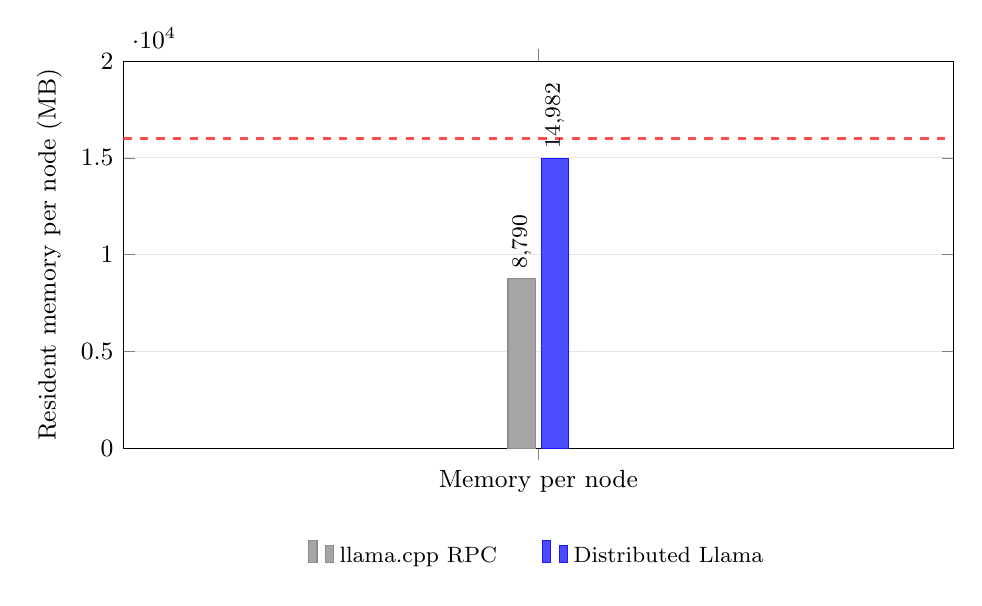
\begin{tikzpicture}
    \begin{axis}[
        ybar,
        bar width=10pt,
        width=\linewidth,
        height=6.5cm,
        enlarge x limits=0.5,
        ymin=0, ymax=20000,
        ylabel={Resident memory per node (MB)},
        symbolic x coords={Memory per node},
        xtick=data,
        xticklabel style={font=\small},
        yticklabel style={font=\small},
        ylabel style={font=\small},
        nodes near coords,
        every node near coord/.append style={
            font=\footnotesize, 
            rotate=90, 
            anchor=west,
            /pgf/number format/fixed,
            /pgf/number format/precision=2
        },
        legend style={
          at={(0.5,-0.22)}, anchor=north,
          legend columns=2, font=\footnotesize, draw=none,
          /tikz/every even column/.append style={column sep=0.5cm},
        },
        ymajorgrids, major grid style={gray!20},
    ]
      \addplot[fill=gray!70, draw=gray!90] coordinates {(Memory per node,8790)};
      \addplot[fill=blue!70, draw=blue!90] coordinates {(Memory per node,14982)};
      
      % --- ADDED: The actual legend command ---
      \legend{llama.cpp RPC, Distributed Llama}
      
      % --- SIMPLIFIED: Draw the 16 GB ceiling line directly ---
      \draw[dashed, red!70, thick] 
        ({rel axis cs:0,0} |- {axis cs:Memory per node,16000}) -- 
        ({rel axis cs:1,0} |- {axis cs:Memory per node,16000});

    \end{axis}
  \end{tikzpicture}
  \caption{Per-node resident memory on Qwen3 14B Q4\_0. Distributed Llama operates within approximately 1~GB of the Raspberry Pi~5's 16~GB ceiling, while llama.cpp RPC retains roughly 7~GB of headroom per node. This is the only metric on which llama.cpp RPC outperforms Distributed Llama, and it is the decisive factor for models beyond the Tier~C scale.}
  \label{fig:rq3-memory}
\end{figure}

This is the only metric that llama.cpp RPC outperformed Distributed Llama at Tier C. llama.cpp RPC used 8.97 GB per node while Distributed Llama used 14.98 GB per node, a 70\% difference. As a result, llama.cpp RPC could accommodate a larger model or much longer context window before OOM. This inverted the per-node memory advantage of Distributed Llama in tier A and B, where its leaner buffer allocation gave it the lower footprint. At tier C, that flipped because Distributed Llama materialized a larger share of weights on each node while llama.cpp RPC distributed the weights more evenly.
\subsection{Summary}
While deciding how to run AI on Raspberry Pi cluster, there is not a single best framework. The choice depends on the model's size and the hardware's memory. Distributed Llama is built for pure speed, generating 85\% faster and putting the CPU to work much more effectively, which makes it a perfect choice for smaller models. Yet, this framework requires a lot more memory to pull off that speed. In contrast, llama.cpp RPC handles the memory much more efficiently by splitting the model layers evenly between nodes. Yet, it is significantly slower due to its processing style, which leaves the CPU sitting idle waiting for the preceding node. 

\subsection{Consistency Check}
\begin{table}[H]
\centering
\caption{llama.cpp: single device vs cluster}
\label{tab:model-breakdown}
\begin{tabular}{lccc}
\hline
\textbf{Model} & \textbf{Exact\%} & \textbf{Avg BLEU} & \textbf{Avg BERT} \\ 
\hline
llama-3.2-1b-instruct-q4\_0 & 0.0\%  & 0.5575 & 0.9512 \\
qwen3-1.7b-q4\_0            & 25.0\% & 0.3058 & 0.8826 \\
qwen3-8b-q4\_0              & 0.0\%  & 0.5174 & 0.9393 \\ 
\hline
\end{tabular}
\end{table}

\begin{table}[H]
\centering
\caption{dllama: single device vs cluster}
\label{tab:model-breakdown-3}
\begin{tabular}{lccc}
\hline
\textbf{Model} & \textbf{Exact\%} & \textbf{Avg BLEU} & \textbf{Avg BERT} \\ 
\hline
llama-3.2-1b-instruct-q4\_0 & 0.0\%  & 0.3343 & 0.9079 \\
qwen3-1.7b-q4\_0            & 0.0\%  & 0.6305 & 0.9480 \\
llama-3.1-8b-instruct-q4\_0 & 50.0\% & 0.7254 & 0.9636 \\
qwen3-8b-q4\_0              & 50.0\% & 0.7436 & 0.9667 \\ 
\hline
\end{tabular}
\end{table}

Tables~\ref{tab:model-breakdown} and~\ref{tab:model-breakdown-3} show what happens when
the same framework runs the same model on one node versus two. The results are interesting since moving from single device to cluster always changes the output, even at the temperature = 0. Specifically, for llama.cpp, exact match was 0\% on two of three models with only Qwen3 1.7B retaining at 25\%. For Distributed Llama, small model's exact match was 0\% while 8B-class models achieved 50\%.

The drop in exact match is expected. Both parallelism mechanisms change the order of floating-point operations. Pipeline offloading introduces serialization and de-serialization of intermediate activations between nodes while tensor parallelism reshapes every layer's matrix multiplication into smaller operations whose results are then combined via all-reduce. Floating point addition is not associative, so a different order when reducing generates different result. At temperature = 0, the model picks the highest probability token at every step, so one small change early on can lead to a completely different output.

What matters is if the differences affect the meaning of the generated outputs or not. The BERTScore results showed they were mostly just wording changes instead, since the scores were high, 0.88 to 0.97. On the other hand, the BLUE scores varied more because a single mismatch token can drop the n\-gram overlap score significantly. Distributed Llama's BLUE scores were higher than llama.cpp in general since the tensor parallelism introduces the numerical differences within each layer rather than across entire layer groups.
\begin{table}[htbp]
\centering
\caption{single device: llama.cpp vs dllama}
\label{tab:model-breakdown-2}
\begin{tabular}{lccc}
\hline
\textbf{Model} & \textbf{Exact\%} & \textbf{Avg BLEU} & \textbf{Avg BERT} \\ 
\hline
llama-3.2-1b-instruct-q4\_0 & 0.0\% & 0.2035 & 0.8982 \\
qwen3-1.7b-q4\_0            & 0.0\% & 0.2137 & 0.8655 \\
qwen3-8b-q4\_0              & 0.0\% & 0.2883 & 0.9141 \\ 
\hline
\end{tabular}
\end{table}


\begin{table}[htbp]
\centering
\caption{cluster: llama.cpp vs dllama}
\label{tab:model-breakdown-4}
\begin{tabular}{lccc}
\hline
\textbf{Model} & \textbf{Exact\%} & \textbf{Avg BLEU} & \textbf{Avg BERT} \\ 
\hline
llama-3.1-8b-instruct-q4\_0 & 0.0\% & 0.1809 & 0.9068 \\
llama-3.2-1b-instruct-q4\_0 & 0.0\% & 0.1515 & 0.9004 \\
qwen3-1.7b-q4\_0            & 0.0\% & 0.2075 & 0.8689 \\
qwen3-14b-q4\_0             & 0.0\% & 0.3243 & 0.9206 \\
qwen3-8b-q4\_0              & 0.0\% & 0.3110 & 0.9101 \\ 
\hline
\end{tabular}
\end{table}

Tables~\ref{tab:model-breakdown-2} and~\ref{tab:model-breakdown-4} compare llama.cpp
against Distributed Llama directly, both in single-device and cluster configurations. The exact match was 0\% across every model in both configurations, and BLEU scores dropped sharply to 0.15--0.32 range. However, BERTScore remained high at 0.87-0.92, which indicates semantic similarity. 

This cross framework divergence was larger than within framework divergence. The reason simply because the two frameworks use different model formats, matrix multiplication routines, memory layouts for weight tensors, orders of operations, etc. Even on a single device with no distribution involved these differences also produce enough numerical drift to make the two frameworks generated different output texts. With cluster configuration, there were extra overheads on top of these baseline differences, and the BLUE scores dropped further as a result.

\subsection{Summary}
Three conclusions follow from these results. Firstly, exact match between a single device and cluster configurations should not be expected even with temperature = 0. Secondly, despite this, the meaning is still preserved. BERTScore above 0.87 shows that outputs stay semantically similar. For IoT tasks like sensor analysis or recommendations, it is still acceptable. Finally, these comparisons should not be used to measure the accuracy of the two frameworks. Neither framework is more accurate than the other.